\apendice{Documentación de usuario}

\section{Introducción}
En este apartado se hablará acerca de los diferentes requisitos de usuario, el proceso de instalación para la aplicación del proyecto y el manual de usuario con el fin de que quede explicado cómo usar la aplicación.

\section{Requisitos de usuarios}
Los requisitos de usuario necesarios son muy sencillos, tan solo es necesario que el usuario disponga de una conexión a internet con la que poder conectarse al \emph{notebook} de Gamma o de \emph{Google Colab}.

Como requisito adicional tendrá que conocer el enlace que le permitiría acceder a dichos \emph{notebooks}.

\section{Instalación}
Para poder disfrutar de la aplicación no es necesaria ninguna instalación en el ordenador del usuario. Tan solo será necesario instalar \emph{Detectron2} en el \emph{notebook} de \emph{Google Colab}, ya que no tiene por defecto la librería necesaria y cada sesión será necesaria su instalación al borrar todos los directorios de la aplicación al finalizar la sesión de \emph{Colab}.

De forma contraria, en Gamma se podrá utilizar la aplicación sin instalar ningún paquete adicional, porque la máquina siempre cuenta con todas las librerías necesarias en el entorno instaladas.

\section{Manual del usuario}
Al poder usar la aplicación desde dos métodos distintos, según donde nos encontremos tendremos un manual de usuario u otro.

\subsection{Google Colab}
Una vez hayamos accedido al \emph{notebook} de \emph{Google Colab} es turno de instalar y descargar todo lo necesario antes de poder utilizar la aplicación. Esto se debe principalmente a que \emph{Google} borra todo el contenido al finalizar sesión y no está instalado \emph{Detectron2} por lo que es necesaria su instalación.

Para poder ejecutar las celdas del \emph{notebook} hay que pulsar al botón circular (Figura \ref{f:play}) que se encuentra al lado izquierdo de cada celda.

\begin{figure}[h]
 \centering
  
\includegraphics[width=0.07\textwidth]{img/Play.PNG}
 \caption{Botón Ejecución Google Colab}
 \label{f:play}
\end{figure}

El primer paso será descargar e instalar \emph{Detectron2} que es un proceso que suele tomar unos minutos. A continuación, se descargan las funciones de la aplicación, subidas al repositorio de \emph{GitHub} del proyecto.

Lo siguiente será importar todas las bibliotecas necesarias para el correcto funcionamiento de la aplicación. También será necesario descargarse el modelo de \emph{Google Drive}, que aunque es pesado, tarda apenas unos segundos en descargarse.

Ahora ya se dispone de todo lo necesario para poder usar la aplicación. Es turno de subir las radiografías, para ello se ejecutará la celda \textbf{Cargar Imagen}. Ahora habrá aparecido un botón (Figura \ref{f:upload}) que permite subir las radiografías a la aplicación.

Finalmente, se ejecutará la celda \textbf{Calcular Longitud}. Tras esperar unos segundos empezarán a aparecer los resultados, formados por la radiografía original, la radiografía segmentada (detección del diente y nervio) y la radiografía con la recta por la cual se ha obtenido su longitud. También, aparecerá un recuadro para cada radiografía con su longitud (Figura \ref{apli}).

\begin{figure}[h]
    \centering
    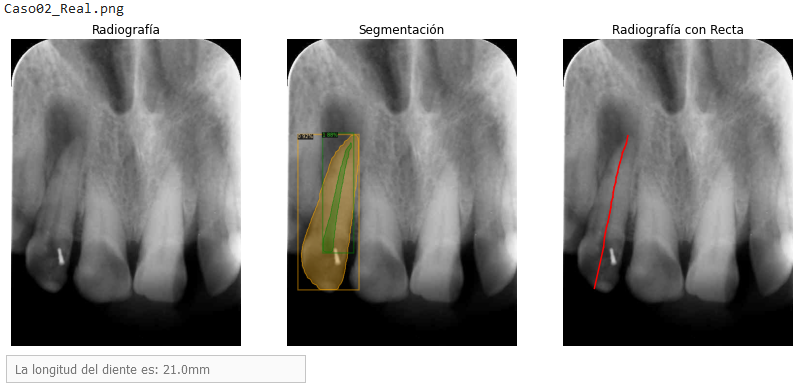
\includegraphics[scale=0.6]{./img/ResultadoApl.png}
    \caption{Resultado Aplicación Final.}
    \label{apli}
\end{figure}

\subsection{Gamma}
Una vez hayamos entrado a \emph{Jupyer Notebook} a través de la herramienta \emph{Ngrok}, hay que dirigirse a la aplicación, que se corresponde al fichero \texttt{Aplicacion.ipynb}.

Una vez nos encontremos en el interior del \emph{notebook} hay que importar todos los paquetes necesarios en la aplicación. Para ello nos colocamos en la primera celda y usaremos el botón del menú superior \textbf{Run}. Una vez se haya terminado de ejecutar, aparecerá a su izquierda el número 1, como se aprecia en la Figura \ref{f:celda1}.

\begin{figure}[h]
 \centering
  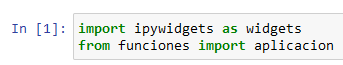
\includegraphics[width=0.6\textwidth]{img/Gamma1.PNG}
 \caption{Ejemplo Ejecución Celda 1 Aplicación}
 \label{f:celda1}
\end{figure}

A continuación, es turno de preparar la subida de las radiografías a la aplicación. Para ello, nos colocamos en la siguiente celda y la ejecutamos de igual manera. Ahora aparecerá un botón, llamado \textbf{Upload} (Figura \ref{f:upload}), que al pulsarlo nos permitirá subir todas las radiografías deseadas.

\begin{figure}[h]
 \centering
  
\includegraphics[width=0.3\textwidth]{img/Gamma2.PNG}
 \caption{Botón Upload}
 \label{f:upload}
\end{figure}

Para poder subir varias radiografías a la vez, es tan sencillo como mantener pulsada la tecla \emph{Ctrl} e ir seleccionando todas las radiografías deseadas.

Una vez se hayan subido las imágenes, aparecerá un mensaje en la celda con los nombres de las radiografías cargadas. Ahora es momento de ejecutar el proceso de cálculo. Para ello, nos vamos a la tercera celda y la ejecutamos. Tras esperar unos segundos empezarán a aparecer los resultados, formados por la radiografía original, la radiografía segmentada (detección del diente y nervio) y la radiografía con la recta por la cual se ha obtenido su longitud.

Finalmente, aparecerá una recuadro indicando la longitud del diente correspondiente a cada radiografía (Figura \ref{apli}).

Por último, sería recomendable cerrar la sesión del \emph{notebook} que acabamos de usar. Para ello, cerramos la pestaña de la aplicación y en el botón de \emph{Running} (Figura \ref{f:running}) saldrá la aplicación. Es tan sencillo como pulsar al botón \emph{Shutdown} (Figura \ref{f:shutdown}) y habremos finalizado toda ejecución en la aplicación. De esta forma se evita que surja cualquier posible problema.

\begin{figure}[h]
 \centering
  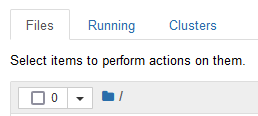
\includegraphics[width=0.4\textwidth]{img/Gamma3.PNG}
 \caption{Botón Running}
 \label{f:running}
\end{figure}

\begin{figure}[h]
 \centering
  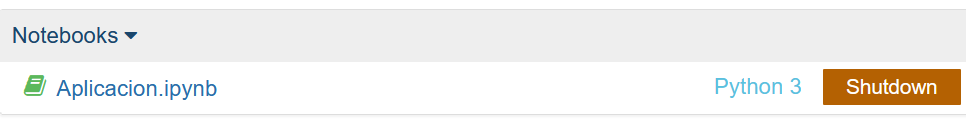
\includegraphics[width=1\textwidth]{img/Gamma4.PNG}
 \caption{Botón Shutdown}
 \label{f:shutdown}
\end{figure}